\chapter{Administration Manual - Platform}
\label{attachments:admin-manual-platform}

\section{Local development}
\label{attachments:admin-manual-local-development}
Local development is essential to test new features and debugging. This section outlines the requirements and steps to set up your local development environment for the platform, ensuring that all components function together seamlessly.


\subsection{Prerequisites}
Before setting up the local development environment, ensure that you have the following prerequisites installed:
\begin{itemize}
    \item \textbf{Node.js $\geq$ 16}
    \item \textbf{Docker}
    \item \textbf{Yarn}
\end{itemize}

\subsection{Running database}
Navigate to the source directory containing the \texttt{docker-compose.yml} file which includes the service definition for the database.
Run the following command to start the service:
\texttt{docker compose up -d}.
This command will pull the necessary images and create container for your database and start the service on the background.

\subsection{Running backend and frontend services}
\begin{enumerate}
    \item Once you have \texttt{yarn} and \texttt{Node.js} installed - preferably by using some package manager like \texttt{asdf}.
    \item Run \texttt{yarn install} to install all the dependencies needed.
    \item Set up a public S3 bucket to upload files from seller configurations. 
    \item Create a \texttt{.env} file and place it in the root folder. The file should contain the following:
\begin{lstlisting}[language=bash,caption={Platform local environment configuration}]
JWT_SECRET_KEY=<key>
JWT_ACCESS_LIFESPAN_SECONDS=3600
JWT_REFRESH_LIFESPAN_SECONDS=604800
AWS_ACCESS_KEY_ID=<access_key_id>
AWS_SECRET_ACCESS_KEY=<secret_access_key>
AWS_SECRET_KEY_ID=<secret_key_id>
PARCELSYNC_AWS_ACCESS_KEY_ID=<parcelsync_access_key_id>
PARCELSYNC_AWS_SECRET_KEY_ID=<parcelsync_secret_key_id>
FROM_EMAIL=<from_email>
AWS_ACCOUNT=<aws_account>
AWS_S3_ASSETS_BUCKET=<s3_bucket_url>
\end{lstlisting}
    \item Run \texttt{yarn start} and all three services (both frontends and API) should start up.
\end{enumerate}
    

\section{Administration Manual - AWS Infrastructure}
\label{attachments:admin-manual-aws-platform}
This section provides a comprehensive guide to managing the platform's AWS infrastructure. 
Although the implementation and integration processes mainly leverage \ac{IaC} for efficiency and consistency, there are instances where manual intervention is required. 
Accessing logs, managing database credentials, and performing specific tweaks often require direct interaction with the AWS Management Console. 
This section outlines essential administrative tasks and highlights adjustments and configurations that were manually implemented during the deployment phase, providing information about how to effectively navigate and manage the AWS environment.

Please note that as long as there is an option, all infrastructure should be deployed within eu-central region.

\subsection{Lambda}
The backend service fully utilises \textit{AWS Lambda} for the deployment and related services. 
This section will describe managing of the Lambda handlers of both backend service and scheduled tasks.


\subsubsection{Accessing logs}
Logs of the Lambda handlers are accessible within the AWS console in \textit{CloudWatch} section.
Here it is possible to list all the log groups within whole account where are all the deployed services as well as Lambda handlers used as scheduled tasks and those ran while deployment (migrations).

To access the logs at a specific time, click the desired log group (usually labelled production environment see Figure \ref{img:admin-manual-aws.lambda.log}) and scroll through the log stream (see Figure \ref{img:admin-manual-aws.lambda.log.detail}) to find the time and event you want (see Figure \ref{img:admin-manual-aws.lambda.log.event.detail}).

\begin{figure}[H]\centering
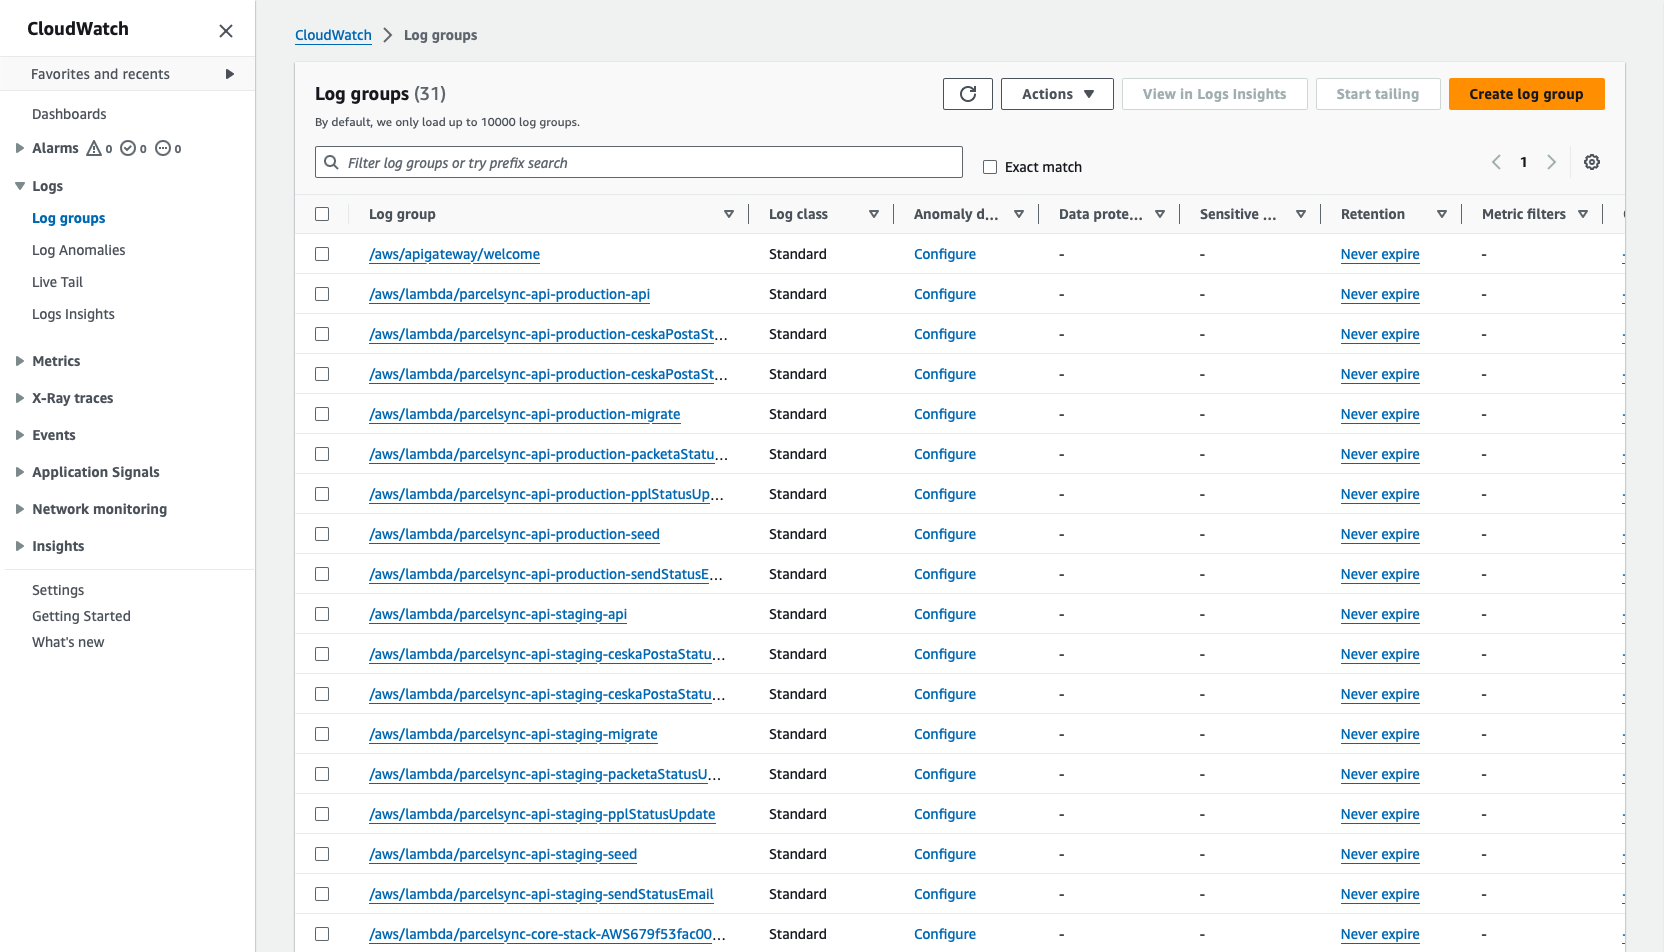
\includegraphics[width=140mm]{img/docs/fig_aws_cloudwatch.png}
\caption{AWS CloudWatch}
\label{img:admin-manual-aws.lambda.log}
\end{figure}

\begin{figure}[H]\centering
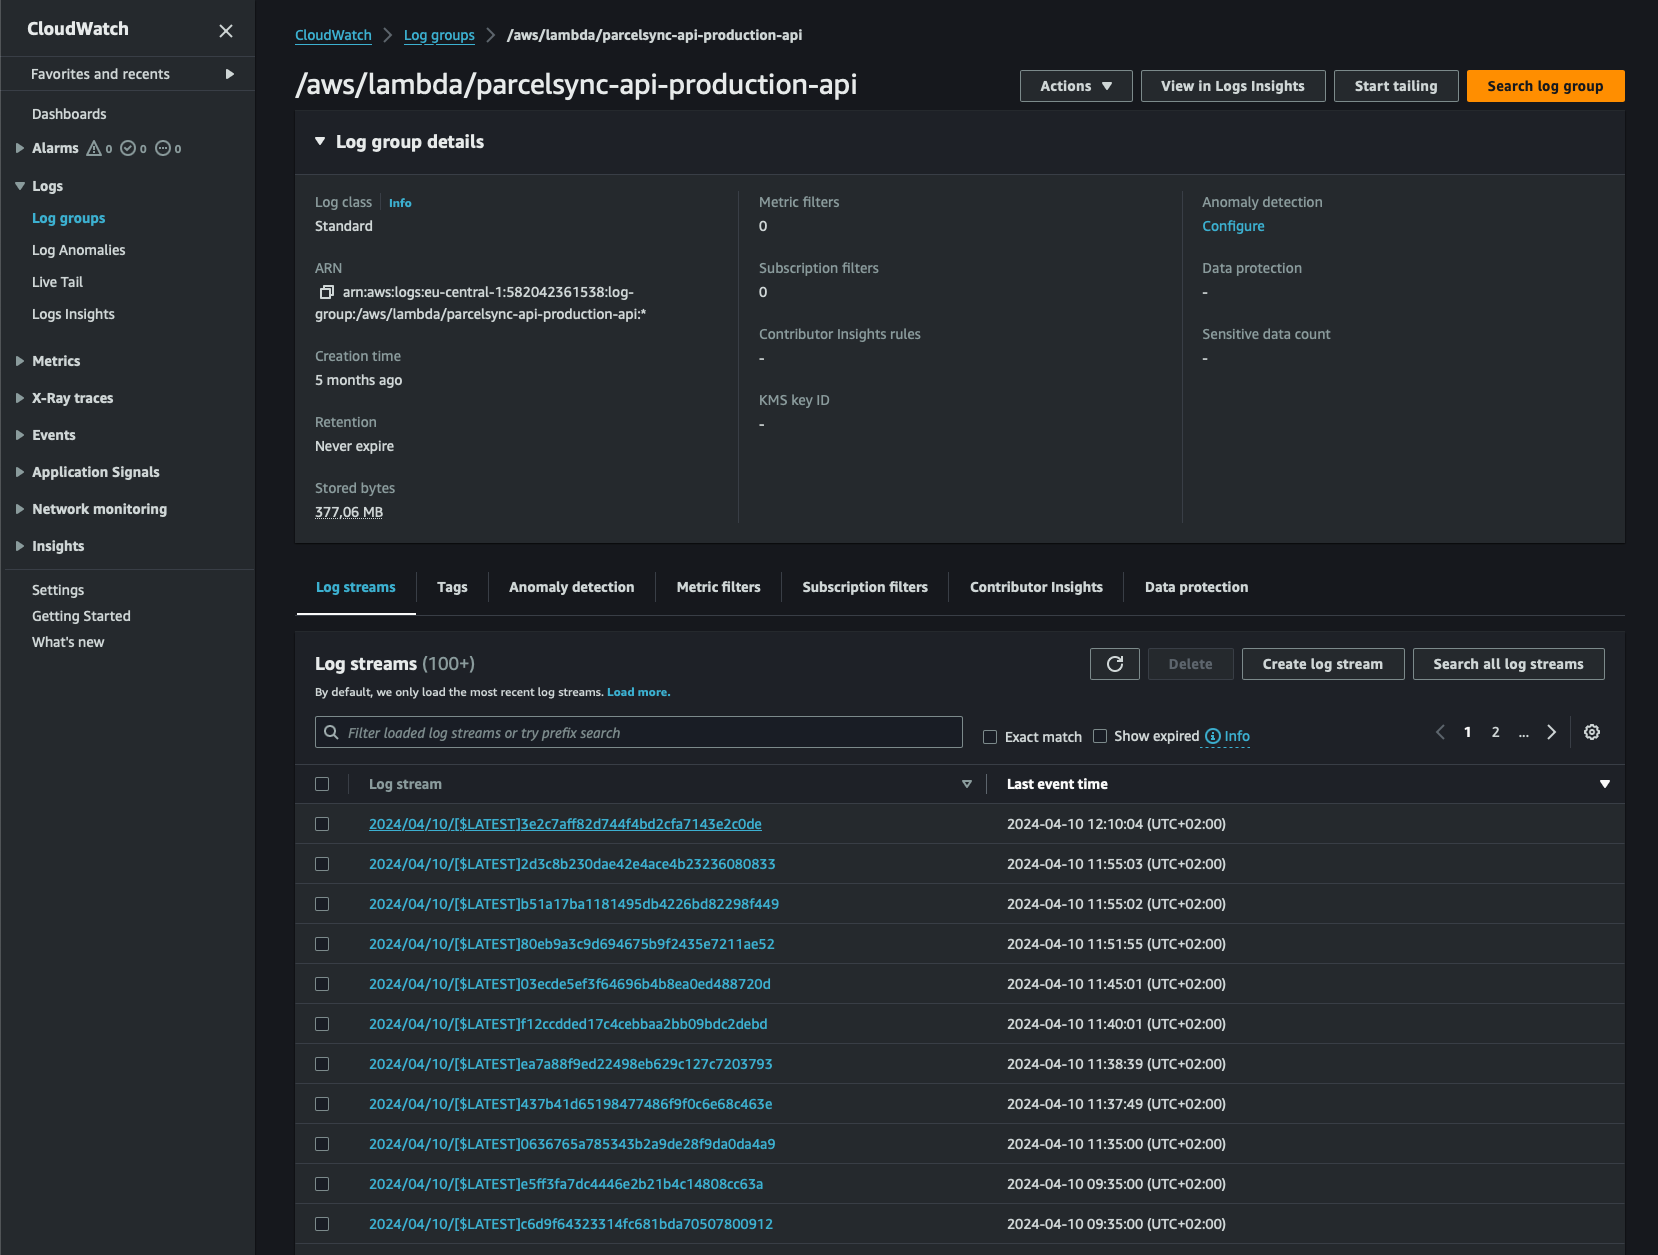
\includegraphics[width=140mm]{img/docs/fig_aws_loggroup.png}
\caption{AWS CloudWatch Log Group detail}
\label{img:admin-manual-aws.lambda.log.detail}
\end{figure}

\begin{figure}[H]\centering
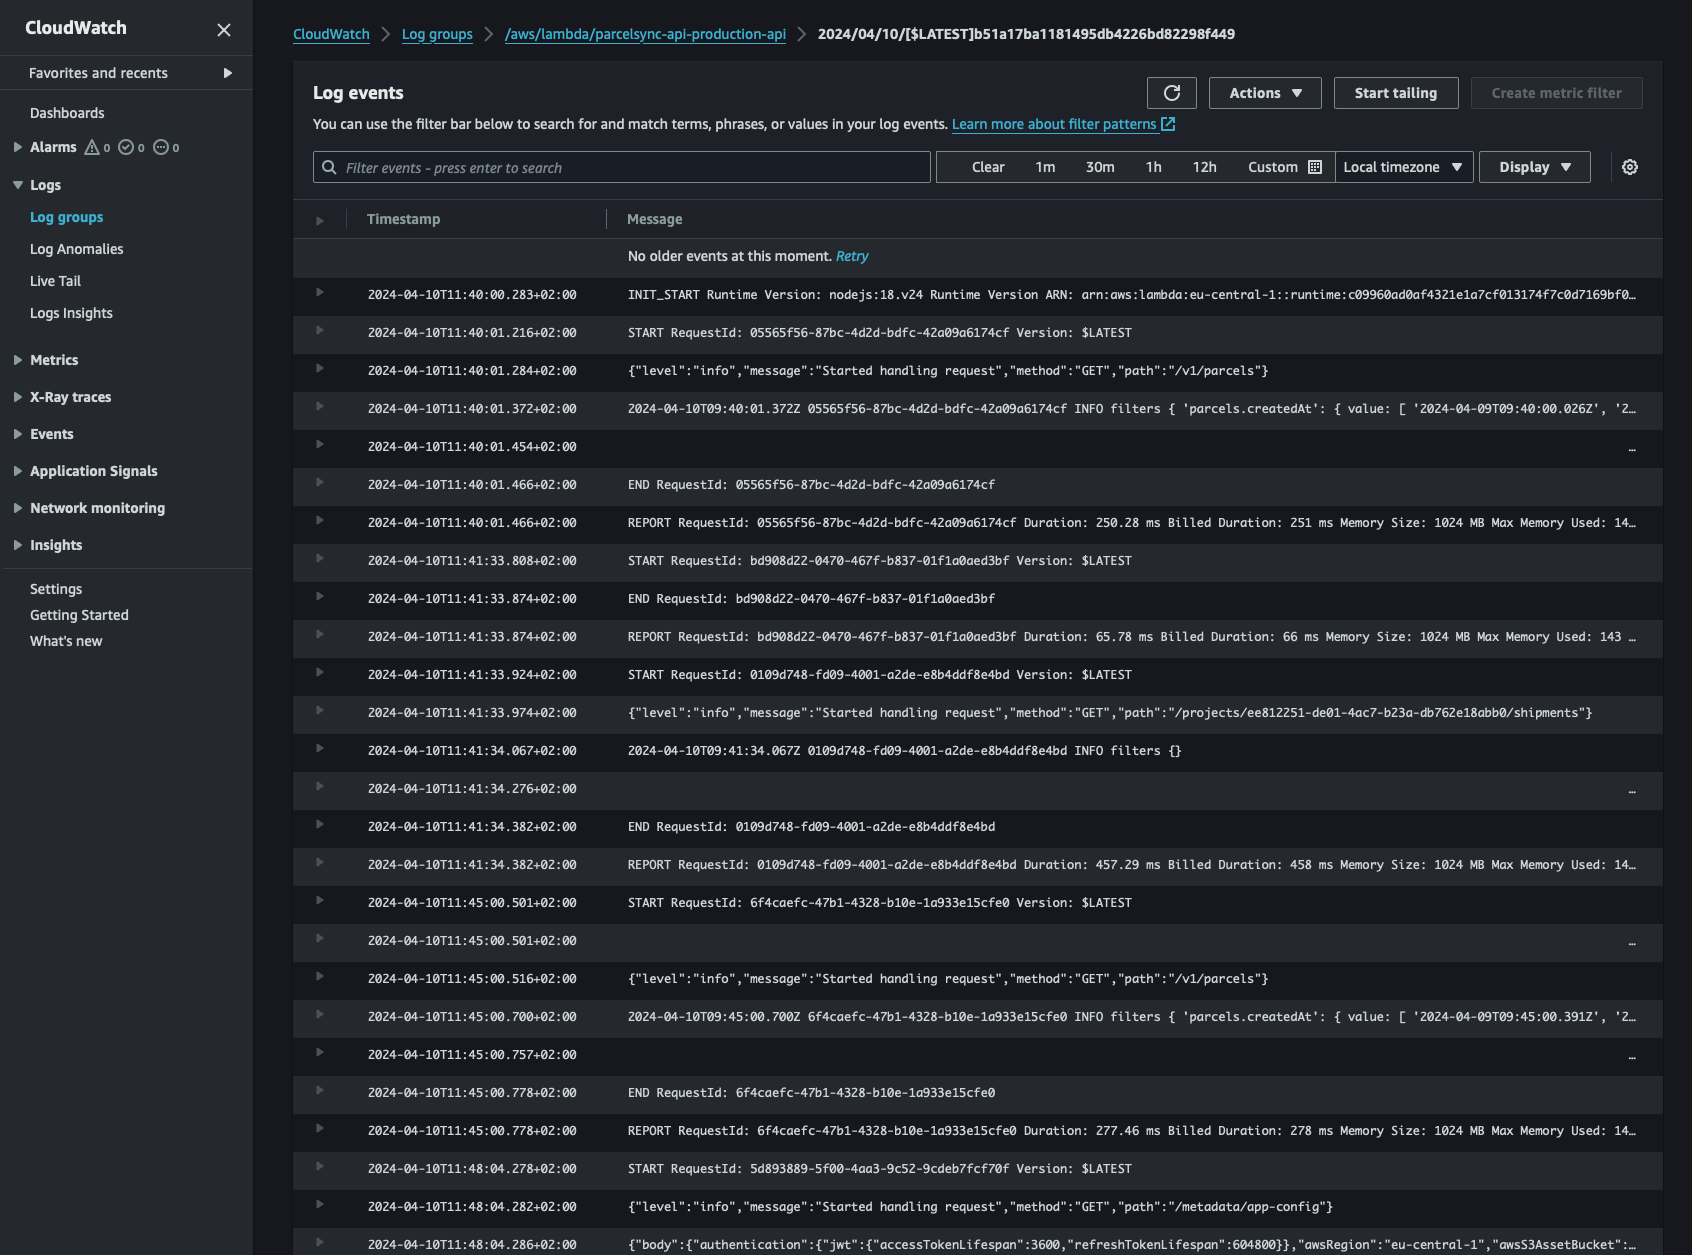
\includegraphics[width=140mm]{img/docs/fig_aws_log_event.png}
\caption{AWS CloudWatch Log Group event detail}
\label{img:admin-manual-aws.lambda.log.event.detail}
\end{figure}

\subsubsection{Scheduled tasks}
\label{attachments:admin-manual-lambda.scheduled-tasks}
Scheduled tasks can be found in the list of all Lambda functions.
They are conveniently named and are used to retrieve shipment status from supported carriers and send tracking emails to customers.
Each of these tasks has \textit{EventBridge} attached with configuration of the event trigger (cron-like definition), see Figure \ref{img:admin-manual-aws.lambda.eventbridge}
We currently use these Lambda functions as scheduled tasks:
\begin{itemize}
    \item \texttt{packetaStatusUpdate}: For Packeta parcel status retrieval.
    \item \texttt{pplStatusUpdate}: For Packeta parcel status retrieval.
    \item \texttt{ceskaPostaStatusRequest}: To request parcel statuses within given timeframe.
    \item \texttt{ceskaPostaStatusPickup}: To pickup requested parcel statuses and update them in the database.
    \item \texttt{sendStatusEmail}: To send-out status e-mails based on seller settings (allowed statuses).
\end{itemize}

\begin{figure}[H]\centering
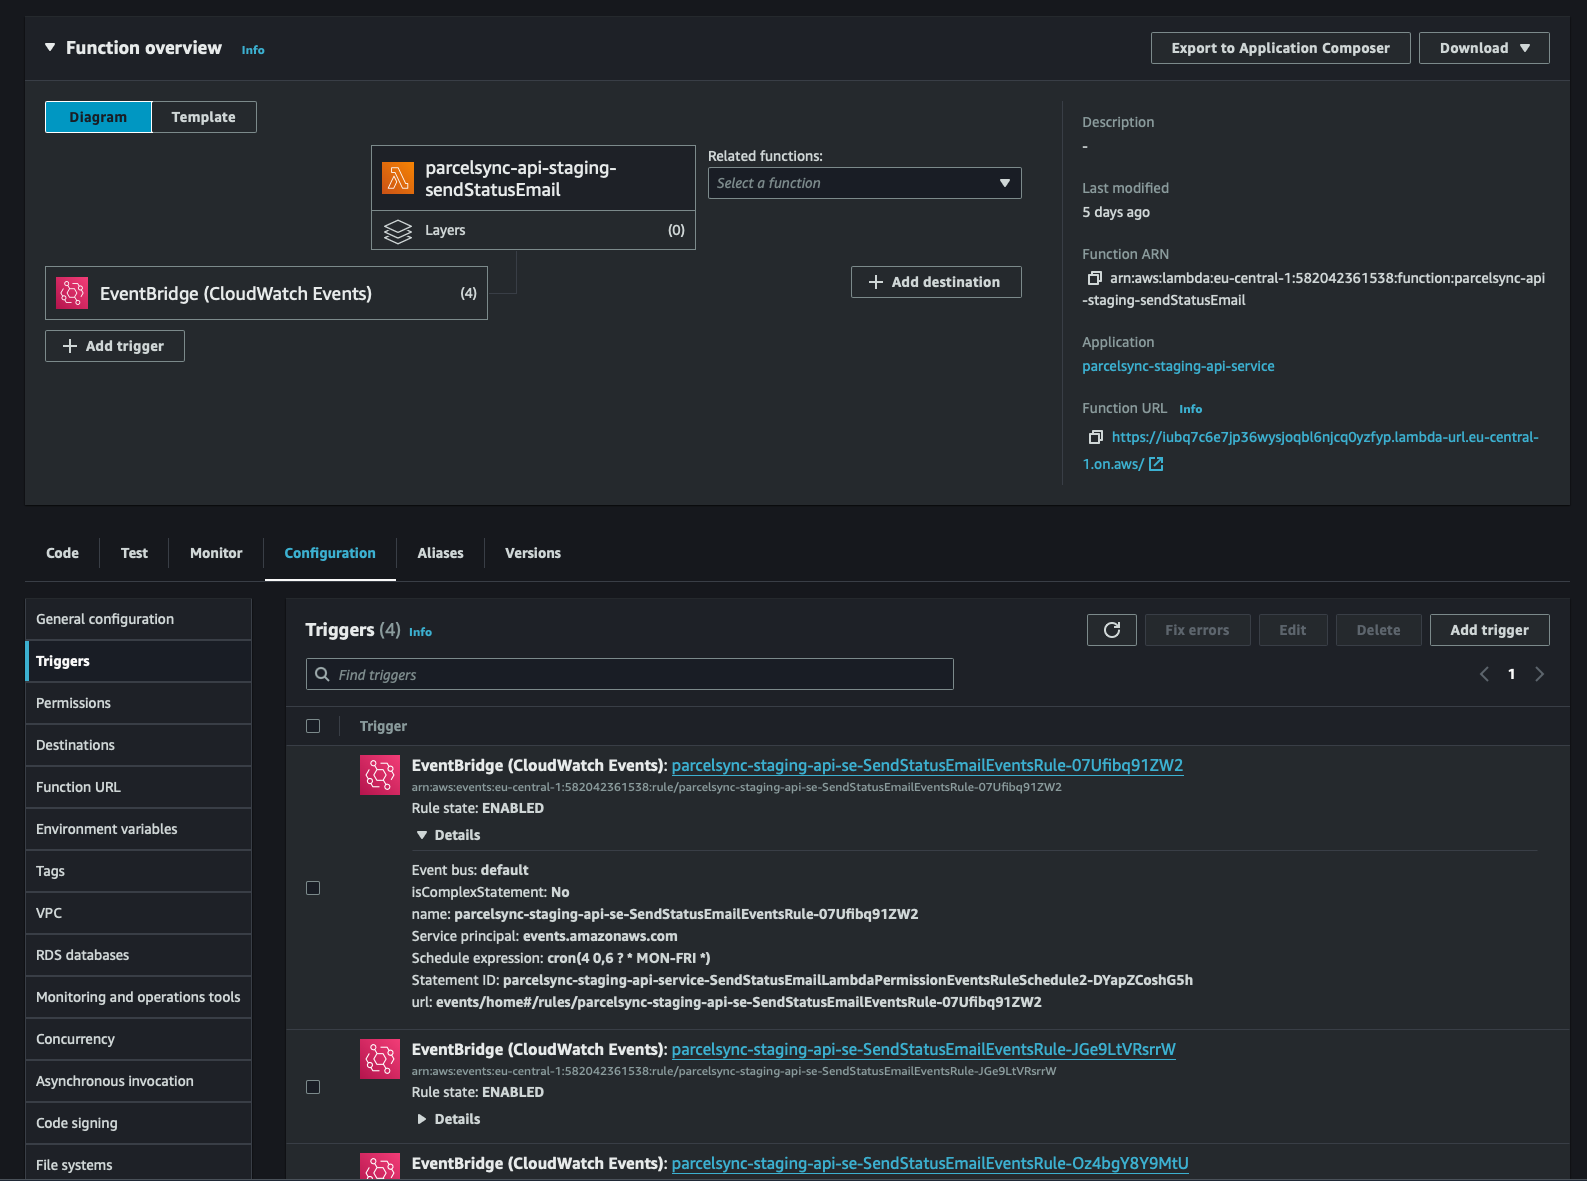
\includegraphics[width=140mm]{img/docs/fig_aws_eventbridge.png}
\caption{AWS Lambda EventBridge definition}
\label{img:admin-manual-aws.lambda.eventbridge}
\end{figure}

\subsubsection{Lambda handler functions}
Lambda handler functions are the entry point methods which are executed when the \texttt{lambda} function is started.
We define the Lambda handler function for all scheduled tasks listed in \ref{attachments:admin-manual-lambda.scheduled-tasks} as well as for the backend service.
Each lambda function can be triggered manually; however, it is recommended to do so only with the scheduled tasks and tasks that run migrations or seeding the database.
You can create the URL of the function in the details of every Lambda function.
This will trigger the function to run, but it is recommended to setup the URL trigger only with \gls{aws-iam} authentication.

Each Lambda function is limited by the predefined timeout of each function.
If the function is time-consuming, we might consider raising the timeout limit from anywhere between 1 second and 15 minutes.
However, bear in mind that the pricing model of the Lambda function relies on billing the execution time.
All our methods are configured with defualt one minute timeouts, except for \texttt{packetaStatusUpdate}.
Due to the large number of Packet packages and the latency of their API responses, we had to extend the timeout to 2 minutes and 30 seconds.
This should be enough because, during the mornings, when the Packeta API tends to be a bit slower, we can update about 600 parcels in approximately 110 seconds.
As soon as the maximum possible time is no longer sufficient, it will be necessary to reconsider the design of the method and decompose it, for example, into Lambda step functions or to use the predefined queue logic used, for example, by the Česká Pošta shipment update.




\subsection{Database}
Database on the AWS is deployed in two instances - staging and production.
Both databases are instances of \textit{Amazon RDS} service setup with the PostgreSQL engine.
The chosen instance type is \texttt{db.t4g.small} \url{https://aws.amazon.com/rds/instance-types/} which was chosen since after testing the \texttt{db.t4g.micro} could not handle a load of 100 sequential Shipment inserts with related objects (to form a complete object) at the same time.

\begin{figure}[H]\centering
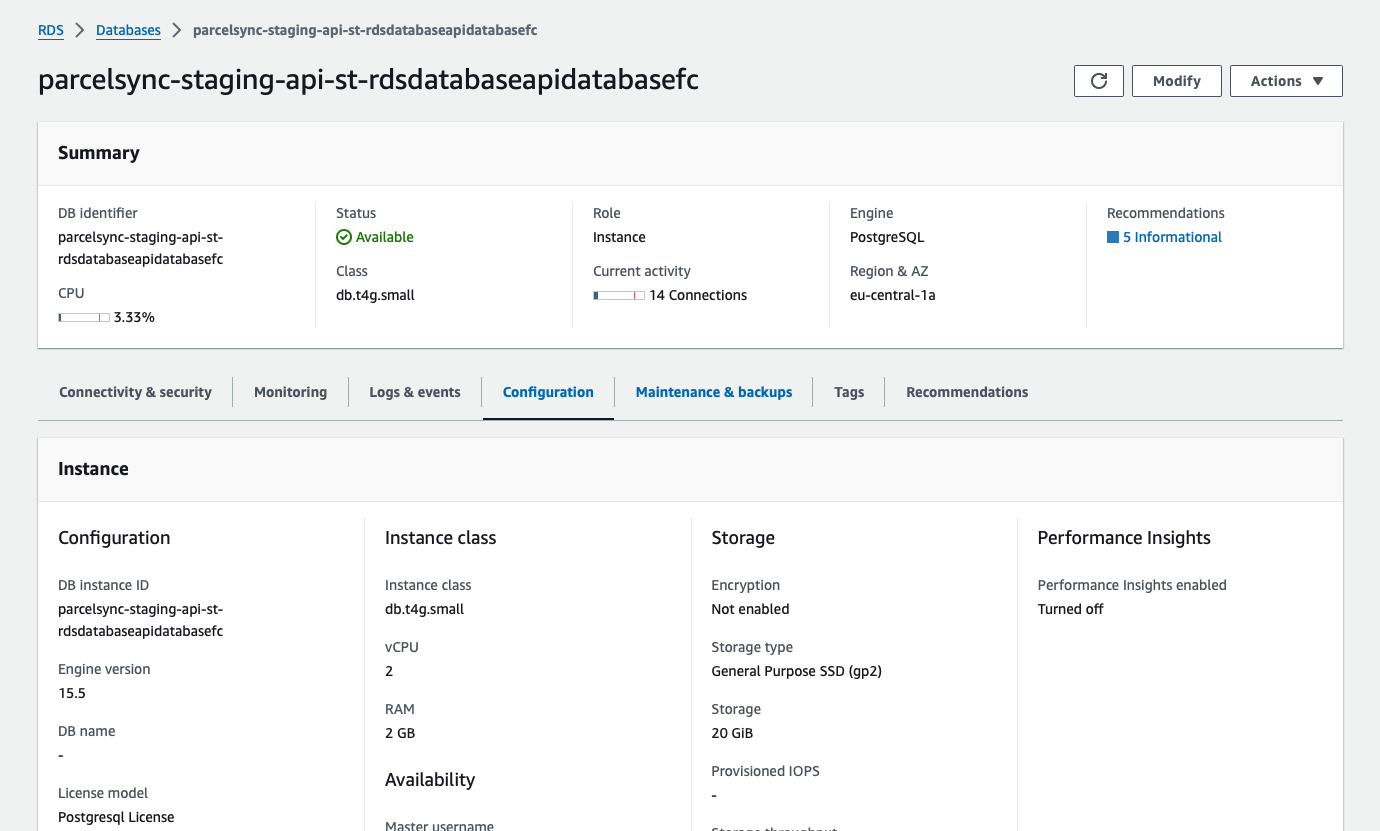
\includegraphics[width=140mm]{img/docs/fig_aws_rds.png}
\caption{AWS RDS instance detail}
\label{img:admin-manual-aws.rds.detail}
\end{figure}

\subsubsection{Accessing credentials}
In order to log into the database from a desktop viewer, it is necessary to obtain the credentials from the console. 
The database credentials of \textit{Amazon RDS} within the AWS console can be obtained in the following way:
\begin{enumerate}
    \item First, log into the AWS console.
    \item From the \textit{Services} menu select \textit{RDS}.
    \item From the database list, select either the staging or production database.
    \item In the \textit{Connectivity \& security} tab can be obtained \textbf{Endpoint} and \textbf{Port} (see Figure \ref{img:admin-manual-aws.rds.detail}.
    \item In the \textit{Configuration} tab, we can see \textbf{Master username}.
    \item To obtain the password, from the \textit{Services} menu select \textit{System Manager}.
    \item In the \textit{Parameter Store} section search for \texttt{DB\_PASSWORD} and choose the expected environment.
    \item In detail, we can show the decrypted value of the password.
\end{enumerate}

\subsubsubsection{Sequential inserts, database pool}
If there are many sequential inserts at the same time from the public API, there is a small chance that all connection slots will be used.

This happened during the testing, and the following was performed:
\begin{enumerate}
    \item Updated \texttt{knex} library used for database connection.
    \item Modified database connection reference to singleton in the lambda API handler.
    \item Upgraded the database instance type to \texttt{db.t4g.small}.
    \item Changed \texttt{max\_connections} parameter in the PostgreSQL database to 1500.
\end{enumerate}

\subsection{\ac{S3}}
\ac{S3} buckets are used to host static exports of frontend applications which are:
\begin{itemize}
    \item User documentation
    \item Tracking page
    \item Dashboard
\end{itemize}

Each of these buckets is served through the \textit{AWS CloudFront} distributions that handle routing.
This \textit{CloudFront} distribution used for the user documentation had to be manually adjusted, more about that in Section \ref{attachments:admin-manual-aws.s3.docs_redirect}.

However, dedicated \ac{S3} buckets are used to store static assets, for example user-uploaded images for the custom layout of the tracking page and notification emails.
More on that later in Section \ref{attachments:admin-manual-aws.s3.permissions}.

\subsubsection{Documentation deployment (locale redirection)}
\label{attachments:admin-manual-aws.s3.docs_redirect}
As mentioned previously, each bucket with direct routing from Route 53 uses the \textit{AWS CloudFront} distribution.
Due to the nature of the user documentation or, more accurately, the routing of non-primary languages in a given application, it was necessary to adjust the \textit{CloudFront} distribution to ensure that other locales can be served without throwing error 404.
Because, the Czech documentation is served on a non-prefixed path in URI such as \texttt{/docs/welcome}, English documentation is served on prefixed path like \texttt{/en/docs/welcome}. 

This meant creating a simple function within the \textit{AWS CloudFront} that (in the background) attaches the \texttt{index.html} file to the end of each URI.

\begin{enumerate}
    \item In the \textit{AWS CloudFront} console select the \textit{Functions} section.
    \item Now, if not created, create a new function as shown in Listings \ref{attachment:admin-platform.listing.cloudformation_function}  named \texttt{indexhtml-appender} with JavaScript runtime.
\begin{lstlisting}[language=javascript,caption={AWS CloudFront function to  append \texttt{index.html} to each URI}]
function handler(event) {
    var request = event.request;
    var uri = request.uri;

    if (uri.endsWith('/')) {
        request.uri += 'index.html';
    } else if (!uri.includes('.')) {
        request.uri += '/index.html';
    }

    return request;
}
\end{lstlisting}
\label{attachment:admin-platform.listing.cloudformation_function}
\item Publish the function and associate it with distribution of documentation.
\end{enumerate}

This function will ensure that the requests of other languages other than the primary one are resolved correctly from the \ac{S3} bucket directories.

\subsubsection{Setting up permissions for assets storage (enable ACLs)}
\label{attachments:admin-manual-aws.s3.permissions}
\ac{S3} used for storing static assets (uploaded from frontend via backend) require manual adjustments in the permission settings and object ownership after being freshly deployed.

\begin{enumerate}
    \item Navigate to the newly deployed AWS \ac{S3} bucket used to store public assets.
    \item Go to the \textit{Permissions} tab and click on \textbf{Edit} button in section \textit{Block public access (bucket settings)}
    \item Here uncheck all the check-boxes listed (\textit{Block all public access} and save changes as in the Figure \ref{:admin-manual-aws.s3.public}.
    \item Now within the \textit{Permissions} tab, scroll down to \textit{Object Ownership} and click the \textbf{Edit} button. 
    \item Here select \textbf{ACLs enabled} and in the \textit{Bucket Ownership} section select \textbf{Bucket owner preferred}. Your setting should look like in Figure \ref{img:admin-manual-aws.s3.acls} and click \textit{Save changes}.
\end{enumerate}

\begin{figure}[H]\centering
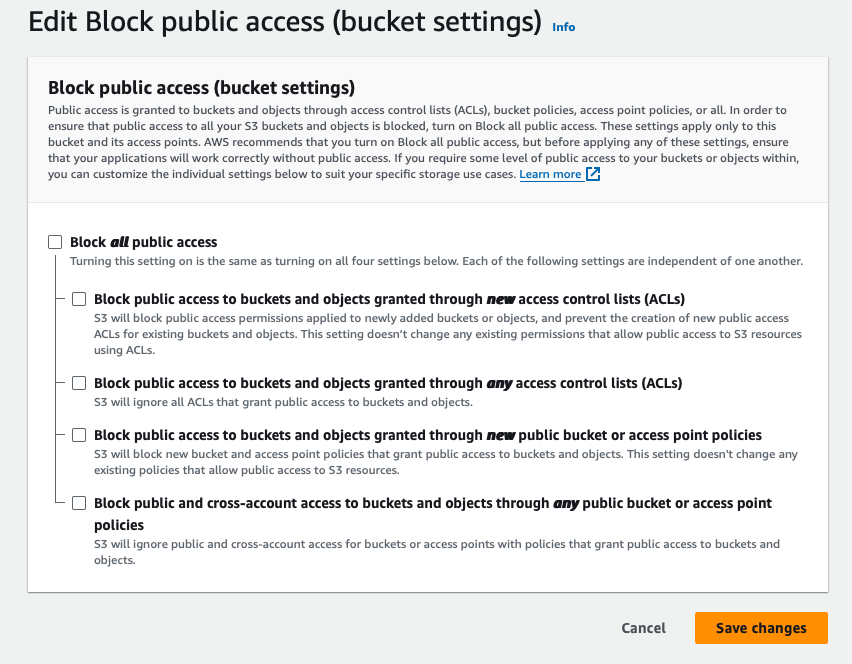
\includegraphics[width=140mm]{img/docs/fig_aws_s3_bucket_public.png}
\caption{AWS S3 bucket Block public access settings}
\label{img:admin-manual-aws.s3.public}
\end{figure}

\begin{figure}[H]\centering
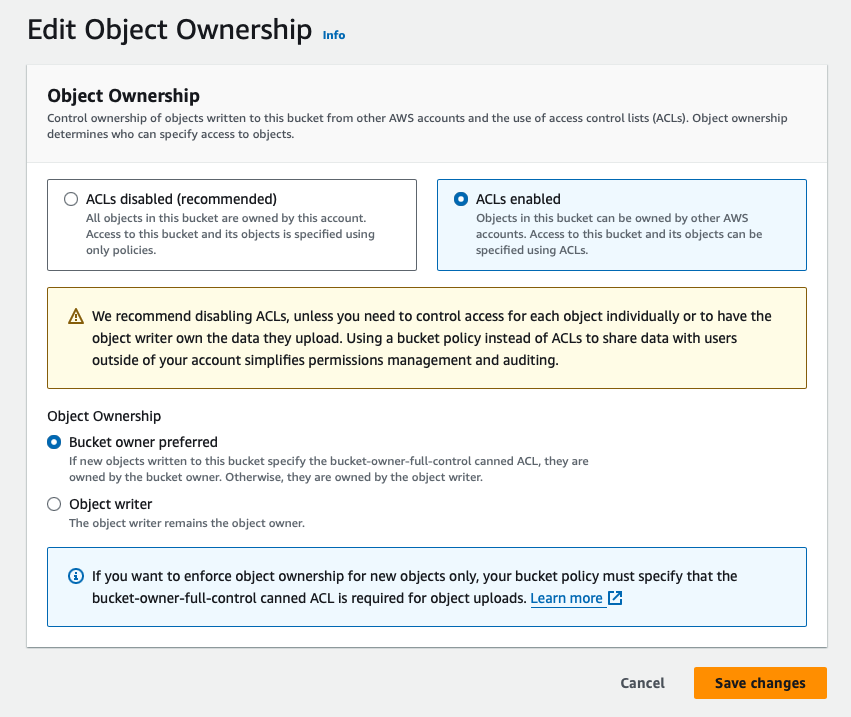
\includegraphics[width=140mm]{img/docs/fig_aws_object_ownership.png}
\caption{AWS S3 bucket object ownership settings}
\label{img:admin-manual-aws.s3.acls}
\end{figure}


\subsection{Email sender}
\label{attachment:ses}
As a email sender service \textit{AWS \ac{SES}} is used.
The account, where the platform is hosted, was moved from the \textit{AWS \ac{SES}} sandbox.
This process took approximately 2 days, and email examples and communication style had to be presented to the AWS support. 
Now the account has a sending quota of 50 000 messages per day with a maximum send rate of 14 messages per second.


\subsection{Deployment to the new AWS account}
% Create new AWS account
% Create IAM user with administration policy
% run yarn aws:setup 
% point domain NS records to the AWS Route53
% run yarn deploy:aws to setup the resources
% % beware of aws account scoring
% push code to the github for the deplyoment of services
Thanks to the complex \ac{IaC} setup within the platform, deployment to the Amazon Web Services is straight forward.
As a prerequisite, you need to have platform repository localy, running {Node.js $\geq$ 16 and have packages installed using \texttt{yarn install} command. 
Create a new clean AWS account \href{https://repost.aws/knowledge-center/create-and-activate-aws-account}{using instructions how to create AWS account} with MFA authentication.
Then follow the \href{https://docs.aws.amazon.com/IAM/latest/UserGuide/id_users_create.html}{instructions how to create IAM user} and use this configuration:
\begin{itemize}
    \item Set password for the IAM user.
    \item Generate Access Key and Secret to allow programatic access.
    \item In the "Set permissions" section, click on "Attach existing policies directly" and select \texttt{AdministratorAccess}.
    \item Skip the "Add tags"
\end{itemize}
Next time you log in to the AWS console, it is recommended to use created IAM.

Now create entry in the \texttt{~/.aws/config} file and append following configuration to the file:
\begin{lstlisting}[language=bash,caption={\texttt{~/.aws/config}}]
[account-name]
region=eu-central-1
output=json
\end{lstlisting}

Now open \texttt{~/.aws/credentials} and using values generated while creating IAM user append the following:
\begin{lstlisting}[language=bash,caption={\texttt{~/.aws/credentials}}]
[account-name]
aws_access_key_id=<ACCES_KEY>
aws_secret_access_key=<SECRET_KEY>
\end{lstlisting}
In order to test the credentials in the CLI, run following command:
\begin{lstlisting}[language=bash,caption={Command to test AWS identity}]
AWS_PROFILE=account-name aws sts get-caller-identity
\end{lstlisting}
This should output JSON with information about the IAM user.

Now, with everything setup locally, it is time to set up the AWS infrastructure.
We will need to setup IAM roles to allow GitHub actions to deploy resources and setup a hosted zone in the Route53 and verify Amazon SES e-mail.
Run the following command:
\begin{lstlisting}[language=bash,caption={Command to setup AWS infrastructure}]
AWS_PROFILE=account-name yarn setup:aws
\end{lstlisting}
Once the task if finished, it will output four name servers.
Add this list of name servers to the domain NS records and wait until the name servers are propagated.
\begin{lstlisting}[language=bash,caption={Command to deploy to the AWS}]
AWS_PROFILE=account-name yarn deploy:aws
\end{lstlisting}

With the services deployed, we need to deploy our applications in the S3 subsets.
For this, it is best to trigger the GitHub deployment action.
Whether in the GitHub repository or by pushing some code to the \texttt{main} branch.

Now continue with Locale redirection on the documentation described in Section \ref{attachments:admin-manual-aws.s3.docs_redirect}, enabling ACLs for assets storage as in Section \ref{attachments:admin-manual-aws.s3.permissions}, and requesting for the SES production access described in Section \ref{attachment:ses}.


